\chapter{Case study}
This chapter studies the practical applicability of ZIO in a development of a server application for Qlik Sense business intelligence tool~\cite{qlik-sense}. First the purpose and the background of the project is introduced along with a quick overview of Qlik Sense. Then, the evaluation of ZIO is divided into several sections, roughly following the structure of Chapter \ref{zio} about ZIO. The first section examines error handling with ZIO and its usability in the development process. The second section discusses the use of dependency injection with ZIO. The third section looks at testing and how ZIO facilitates the implementation of automated tests. The fourth section covers the role of ZIO's concurrency constructs in the development of the application. The last section analyzes the overall usability of ZIO in application development.

The application under study is the backend for a web application. It exposes its functionality via an HTTP interface. The purpose of the application is to manage control parameters of the Qlik Sense business intelligence tool. A browser-based user interface has also been developed for the application, but it is not within the scope of this thesis.

Qlik Sense is a data analytics software with Extract, Transform and Load (ETL), data modeling and interactive data visualization capabilities. Qlik Sense is commonly used to create dashboards that display data from various sources in a single easy-to-consume format. The user of the dashboard can filter the data and export reports in various formats, such as PDF or Excel, or via email message. Qlik Sense has various deployment options including on-premises servers, Kubernetes and more recently also a Cloud/SaaS offering.

It is often desirable to parameterize the operation of Qlik Sense applications, such as URLs, calculation formulas and titles to display. However, Qlik does not have a built-in mechanism to maintain such configurations, and many Qlik applications end up managing configurations in an Excel file or similar. This method is often perceived as suboptimal due to usability challenges for non-technical users, limited possibilities to manage user rights, and deficiencies in validating the correct structure of the configuration, which makes it error prone. A table as a configuration format is also limited in describing, for example, object or array structures.

For these reasons, a custom web application for managing Qlik Sense configuration was developed. The custom solution exposes a HTTP/JSON API that Qlik Sense applications can read configuration values from. Authentication is implemented with an API key, which is simply a token provided by the client in the HTTP headers. The configuration format and values can be managed from a graphical user interface by Qlik application developers.

The code of the application was divided roughly into three layers/modules: core, persistence and HTTP. The core contains all the business logic and interface definitions that are implemented in the persistence layer. The HTTP layer is responsible for exposing the public API of the application. This requires decoding HTTP requests and handling authentication logic. The persistence layer implements interfaces defined by the core and HTTP layers. It translates domain models into relational format and communicates with PostgreSQL database, which is used for persistence.

The application utilizes many libraries from the ZIO ecosystem: zio-protoquill for database interaction, tapir with zio-http for the HTTP server, zio-json for JSON (de)serialization, zio-config for reading and parsing the application configuration, zio-logging for logging and zio-test with zio-testcontainers for testing. The server application is packaged as a Docker container to accommodate the different deployment options of Qlik Sense.


\section{Error handling}
The ZIO error model was proven to be suitable for many situations. Due to the greenfield nature of the project, the development process involved a significant amount of experimentation and refactoring. Changes could be done with confidence because of statically typed errors that trigger a compile error if an error case was accidentally left unhandled. Adding a new error case to a method is easy because the compiler errors indicate where additional error handling is required.

Converting errors between different layers of the application turned out to be easy and convenient. \refsource{casestudy:converterrors} contains part of the \inlinecode{ApikeyRepository} implementation that stores API keys in a PostgreSQL database. Because every API key value must be unique, adding a new API key can fail if the database already contains an API key with the same value. The possibility of failure is reflected in the return type of the \inlinecode{add} method: \inlinescala{IO[DuplicateApikey, Unit]}. Running an insert query against the database can fail with \inlinecode{SQLException}, which must be converted to \inlinecode{DuplicateApikey} or to a ZIO defect, depending on the specific \inlinecode{SQLException} received. The \inlinecode{catchAll} operator expresses this logic clearly.

\begin{algorithm}

\begin{minted}{scala}
class PostgresApikeyRepository(datasource: DataSource):
  def add(apikey: Apikey): IO[DuplicateApikey, Apikey] =
    // Prepare the insert query, implementation omitted for brevity
    val insertApikeyQuery: Query[Apikey] = ???

    // Run the query against a database
    val queryResult: IO[SQLException, Unit] = run(insertApikeyQuery)

    // Convert the SQLException to DuplicateApikey error or defect
    val uniqueViolationHandled: IO[DuplicateApikey, Unit] =
      queryResult
        .catchAll {
          case exc: SQLException if isUniqueViolation(exc) =>
            ZIO.fail(DuplicateApikey(apikey))

          case otherSqlExc: SQLException => ZIO.die(otherSqlExc)
        }

    // Return the original apikey after insert was successful
    uniqueViolationHandled.as(apikey)

  private def isUniqueViolation(exc: SQLException): Boolean =
    exc.getSQLState == PSQLState.UNIQUE_VIOLATION.getState
\end{minted}

\caption{Expressing the desired error handling behavior with \inlinecode{catchAll} operator. \label{casestudy:converterrors}}
\end{algorithm}

Retrying capabilities of ZIO also proved to be useful. The data model for API key contains a secret token and a description. In the application \inlinecode{ApikeyService} is responsible of creating a new API key. The user can specify a description for the key and \inlinecode{ApikeyService} is responsible of creating a token and persisting the new API key. The process of creating a new API key consists of validating that the provided description meets its requirements, generating a new token, persisting the new API key and finally returning the created and persisted API key. The service delegates the creation of the token to \inlinecode{KeyGenerator} and persistence to \inlinecode{ApikeyRepository}.

\begin{algorithm}

\begin{minted}{scala}
class ApikeyService(keyGen: KeyGen, repo: ApikeyRepository):
  def create(description: String): IO[InvalidDescription, Apikey] =
    type CreateError = DuplicateApikey | InvalidDescription

    val createApikey: IO[CreateError, Apikey] = for
      validDesc   <- validateDesc(description)
      token       <- keyGen.generateKey
      savedApikey <- repo.add(Apikey(validDesc, token))
    yield savedApikey

    // Retry only in the case of DuplicateApikey and at most 10 times
    val policy = Schedule.recurWhile[CreateError] {
      case DuplicateApikey(_)    => true
      case InvalidDescription(_) => false
    } && Schedule.recurs(10)

    // Apply the retry policy to the ZIO that creates the apikey
    val retried: IO[CreateError, Apikey] = createApikey.retry(policy)

    // Change the error type of the retried ZIO:
    // IO[CreateError, Apikey] => IO[InvalidDescription, Apikey]
    // By converting all errors to defects except InvalidDescription
    retried.refineOrDieWith {
      case descError: InvalidDescription => descError
    }(otherErr => RuntimeException(s"Defect in create: $otherErr"))

  def validateDesc(str: String): IO[InvalidDescription, String] = ???
\end{minted}

\caption{Expressing sophisticated retry policies declaratively with \inlinecode{Schedule} and \inlinecode{retry} operator on ZIO. \label{casestudy:retries}}
\end{algorithm}

As demonstrated in \refsource{casestudy:converterrors}, persisting the API key can fail if the token already exists in the database. A desired way to react to this situation is by creating a new token and trying to persist the API key again with the new token. However, it is desirable not to retry persisting a new API key indefinetely. If persisting a new API key fails a couple times in a row with \inlinecode{DuplicateApikey}, there is probably a bug in the code, and it should be considered as a defect. \refsource{casestudy:retries} shows the \inlinecode{ApikeyService.create} method that implements the above logic with ZIO. A ZIO \inlinecode{Schedule} describes the retry policy and \inlinecode{refineOrDieWith} is used to convert \inlinecode{DuplicateApikey} to defect if retries do not resolve the error.


\section{Dependency injection}
The services in the application were implemented by using constructor-based dependency injection. If a service requires another service, it will receive the dependency as a constructor argument. This pattern can be seen in Listings \ref{casestudy:converterrors} and \ref{casestudy:retries} where dependencies are received as constructor arguments. Each service defines a \inlinecode{ZLayer} in its companion object, which can be used to construct that specific service. Dependencies for the program are provided in the main method by referencing \inlinecode{ZLayer} of each required service. \refsource{casestudy:dependencyinjection} demonstrates how the layers are provided.

ZIO resolves and constructs the dependency graph at compile time, as described in Section \ref{zio:environment:zlayer}. If a required dependency is not provided, ZIO reports a developer-friendly error message explaining what dependency is missing. This compile time verification proved to be valuable in the development process when new dependencies were added to services. Forgetting to provide a newly-added dependency was brought to the attention of the developer in a clear format before the application could even be started. This can be demonstrated, for example, by commenting out \inlinecode{KeyGen.layer} and \inlinecode{Database.dataSourceLayer} from \refsource{casestudy:dependencyinjection}. The compiler reports an error shown in Figure \ref{fig:zlayer-provide-error}, which clearly states what dependencies are missing and which services require them.

\begin{algorithm}

\begin{minted}{scala}
object Main:
  // Represents the whole program before its dependencies are provided
  val program: ZIO[ApikeyService, Nothing, Unit] = ???

  val run: ZIO[Any, Nothing, Unit] = program.provide(
    ApikeyService.layer,
    PostgresApikeyRepository.layer,
    KeyGen.layer,
    Database.dataSourceLayer,
  )
\end{minted}

\caption{Dependencies are provided in the main method of the application as \inlinecode{ZLayer}s. \label{casestudy:dependencyinjection}}
\end{algorithm}

\begin{figure}[ht!]
    \centering
    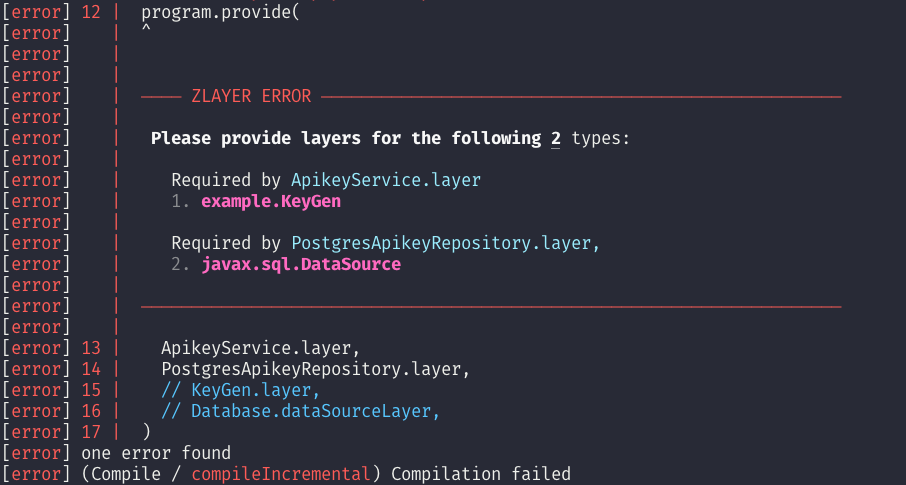
\includegraphics[width=\textwidth]{images/zlayer-provide-error.png}
    \caption{Error message produced by ZIO when required \inlinecode{ZLayer} is not provided.}
    \label{fig:zlayer-provide-error}
\end{figure}


\section{Testing}
The application contains several automated tests. ZIO has its own test library, zio-test, which was used for testing. Three types of tests were written for the application: unit tests, integration tests and system tests. Unit tests run in-memory and exercise a single class or function. Integration tests ensure the correct functionality of multiple services together and may include out-of-process dependencies such as databases. Repository classes that interact with a PostgreSQL database were tested with integration tests that used a database instance running in a Docker container. In system tests the application is tested as a whole, which in this case means that the configuration is read from environment variables and the database is running in a Docker container, similar to integration tests. System tests treat the application as a black box and tests only interact with its public API, which in this case consists of the HTTP endpoints.

Dependency injection in zio-test is managed with \inlinecode{ZLayer}s. This makes it easy to configure tests in a way that the class under test can be provided with fake implementations of its dependencies. ZIO has also built-in \emph{test services} that make it possible to write deterministic tests that interact with the console, time/clock, random number generator and environment variables. This ability to effortlessly test interaction with time and environment variables in a controlled manner proved to be valuable.

\refsource{casestudy:testclock} shows a test for \inlinecode{ApikeyService} that verifies that the revokation time of an API key is set to the current time. In the test a \inlinecode{TestClock} is used to fix the current time visible to the service, and then assert that the hardcoded time was actually used. The example also demonstrates how layers are used to provide dependencies to the class under test.

\begin{algorithm}

\begin{minted}{scala}
test("revoke should set current time as the revokation time") {
  val fixedTime: Instant = Instant.parse("2023-03-30T19:34:28Z")

  for
    apikeyService <- ZIO.service[ApikeyService]
    apikey        <- apikeyService.create("test apikey description")

    _ <- TestClock.setTime(fixedTime) // Set current time
    _ <- apikeyService.revoke(apikey) // Perform logic under test

    // This is verifiable using the provided in-memory repository
    allApikeys    <- FakeApikeyRepository.getAll
    revokedApikey <- ZIO.getOrFail(allApikeys.find(_ == apikey))

  // Assert that the fixed time was used as the revokation time
  yield assertTrue(revokedApikey.isRevokedAt(fixedTime))
}.provide(
  ApikeyService.layer,
  FakeApikeyRepository.layer,
  FakeKeyGen.layer,
) // Test is configured with real ApikeyService and fake dependencies
\end{minted}

\caption{ZIO \inlinecode{TestClock} facilitates testing of code that uses the current time. \inlinecode{ZLayers} enable to inject desired dependencies to the service under test. \label{casestudy:testclock}}
\end{algorithm}

The biggest advantage of ZIO test services were the possibility to configure the environment variables in system tests. The application reads its configuration, such as database connection string and HTTP port number, from environment variables. Traditionally testing how a program interacts with environment variables is cumbersome and error prone to say the least. ZIO \inlinecode{TestSystem} allows to set environment variables easily before the application is started and it tries to read its configuration. \refsource{casestudy:testsystem} shows a layer that requires environment variables that will be set before the application is started and kept running in the background.

\begin{algorithm}

\begin{minted}{scala}
case class EnvVars(values: Map[String, String])

object SystemTestSetup:
  // This layer starts the application in the background and
  // configures it by setting environment variables before starting.
  val layer: ZLayer[EnvVars, Nothing, Unit] =
    TestSystem.default >>> ZLayer.scoped {
      for
        envVars <- ZIO.service[EnvVars]
        _       <- setEnvironmentVariables(envVars)
        _       <- startApp
      yield ()
    }

  // The application keeps it running while tests are finished.
  // Delay makes sure the application has had time to start.
  def startApp = Main.run.forkScoped *> ZIO.sleep(2.second)

  def setEnvironmentVariables(envVars: EnvVars) =
    ZIO.foreachDiscard(envVars.values) { (key, value) =>
      TestSystem.putEnv(key, value)
    }
\end{minted}

\caption{ZIO \inlinecode{TestSystem} makes it possible to set/overwrite environment variables the application sees. This is used to set the configuration for the application in system tests. \label{casestudy:testsystem}}
\end{algorithm}

ZIO test services do not provide a way to control access to the file system, which is also quite hard to test because of similar reasons as environment variables. Even though the application in its current form does not use the file system, it would be nice if ZIO provided tools to test such interactions.


\section{Concurrency}
The application in its current form is quite simple, and thus ZIO's concurrency features were not needed much. This is partly due to the decision to use a relational database, which can perform complex query logic in a single query. In other projects of similar complexity, the need for concurrency typically arises when fetching data from multiple sources and combining the data in the application code. This occurs, e.g, with NoSQL databases, which are usually not capable of doing joins in the database, thus forcing the joining logic to be expressed in the application code.

As the application advances, and we foresee that concurrency plays a more significant role and ZIO's concurrency features will likely become even more useful, especially when the application gains other functionalities besides a HTTP interface. Such features could include scheduled batch jobs running in the background, such as updating and invalidating caches or reporting metrics, or asynchronous messaging where the application must listen to new messages in the background and react accordingly. ZIO's concurrency and scheduling capabilities are well suited for these kind of use cases.


\section{Analysis}
The case study revealed that using ZIO may initially slow down development, but this is only temporary and lasts for days or about one week. While the simplest tasks may sometimes be slightly more challenging to implement with ZIO, the benefits become apparent when dealing with more complex problems. The use of ZIO made it easier to tackle more difficult problems that may typically be ignored in imperative languages due to the time and effort required to solve them, such as examples in Listings \ref{casestudy:converterrors} and \ref{casestudy:retries} demonstrate. Some tasks that are unreasonably difficult (or even practically impossible) in mainstream languages are possible, often simple, with ZIO.

Acknowledging the ever changing and unpredictable nature of software projects, building new projects on strong foundations is desirable. This increases the likelihood that customizing and evolving the software is possible with reasonable effort. In our small experiment, ZIO proved to be a robust foundation that enables such customizations. Refactoring was easy and could be done with confidence because ZIO programs are referentially transparent.

Developers with no previous experience with monadic effects or effects as values may find it difficult to comprehend programs written with ZIO. This became clear in discussions with other developers involved in the project. The programmer must master quite a bit of functional programming techniques and adopt a functional mindset in order to use ZIO (or other monadic effects) effectively.

\new{
One of the key benefits of monads is their ability to describe different aspects of the control flow in a clear and modular manner. Monads facilitate good separation of concerns by allowing developers to define the core business logic, often referred to as "happy path", separately from error handling and concurrency concerns. This separation of concerns facilitates writing maintainable and scalable code. In contrast, the imperative paradigm often conflates these concerns, making it challenging for programmers to focus on one aspect at a time.
}
